\documentclass[10pt, a4paper]{article}

% ==================== Package Imports ====================
\usepackage[utf8]{inputenc}
\usepackage[T1]{fontenc}
\usepackage[english]{babel}
\usepackage{amsmath, amssymb, amsthm}
\usepackage{graphicx}
\usepackage{booktabs}
\usepackage{geometry}
\usepackage{hyperref}
\usepackage{float}
\usepackage{caption}
\usepackage{subcaption}
\usepackage{lipsum}
\usepackage{url}
\usepackage{enumitem}

% ==================== Page Layout ====================
\geometry{
    a4paper,
    left=25mm,
    right=25mm,
    top=25mm,
    bottom=25mm
}

% ==================== Hyperref Setup ====================
\hypersetup{
    colorlinks=true,
    linkcolor=blue,
    filecolor=magenta,      
    urlcolor=cyan,
    pdftitle={From Expansion to Compression: Adaptive Multi-View Recommendation with LLM-based Semantic Denoising},
    pdfauthor={Author Name},
    pdfsubject={Recommendation Systems},
    pdfkeywords={Recommendation, LLM, Graph Neural Networks, Multi-View Learning}
}

% ==================== Theorem Environments ====================
\newtheorem{theorem}{Theorem}
\newtheorem{lemma}{Lemma}
\newtheorem{proposition}{Proposition}
\newtheorem{corollary}{Corollary}
\newtheorem{definition}{Definition}
\newtheorem{example}{Example}
\newtheorem{remark}{Remark}

% ==================== Custom Commands ====================
\newcommand{\RRF}{\textsc{RRF}}
\newcommand{\ASCRec}{\textsc{ASC-Rec}}
\newcommand{\StructCLR}{\textsc{StructCLR}}
\newcommand{\SASRec}{\textsc{SASRec}}
\newcommand{\EASE}{\textsc{EASE}}
\newcommand{\BMtwoFive}{\textsc{BM25}}
\newcommand{\UserKNN}{\textsc{UserKNN}}
\newcommand{\CoRAL}{\textsc{CoRAL}}
\newcommand{\ICL}{\textsc{ICL}}
\newcommand{\ReACT}{\textsc{ReAct}}

% ==================== Document Start ====================
\begin{document}

% ==================== Title Section ====================
\title{From Expansion to Compression: Adaptive Multi-View Recommendation with LLM-based Semantic Denoising}
\author{Anonymous Author}
\date{}

\maketitle

% ==================== Abstract ====================
\begin{abstract}
Graph-based Collaborative Filtering (CF) and Large Language Models (LLMs) represent two distinct paradigms in recommendation, yet they suffer from complementary limitations: CF models are semantically blind to content-driven user intents, while LLMs lack population-level collaborative priors and are prone to hallucinations (e.g., sycophancy). Naively integrating them often leads to negative transfer, where semantic noise dilutes structural precision. To resolve this dilemma, we propose \ASCRec{} (Adaptive Structural-Semantic Cascade), a novel framework operating on an ``Expansion-Compression'' paradigm.

In the Expansion phase, we construct a heterogeneous expert pool spanning structural, statistical, and semantic views. An Attention-based Dynamic Router acts as an adaptive gatekeeper, capturing diverse user states (e.g., cold-start vs. active) to retrieve a broad, high-quality candidate reservoir. In the Compression phase, we treat the LLM not as a direct ranker, but as a Semantic Denoiser. We introduce a Conditional Reciprocal Rank Fusion (Conditional RRF) strategy that leverages LLM-generated reasoning to validate candidates. Crucially, this mechanism applies ``soft demotion'' to items flagged as irrelevant, suppressing noise without discarding valid structural signals. Extensive experiments on three real-world datasets (Amazon Beauty, Sports, and Toys) demonstrate that \ASCRec{} significantly outperforms state-of-the-art baselines. Notably, analysis of information density reveals that our approach successfully shifts the ``Golden Ratio'' of relevant items from the tail to the head of the ranking list, maximizing recommendation utility within limited exposure slots.
\end{abstract}

% ==================== Keywords ====================
\noindent\textbf{Keywords:} Recommendation Systems, Large Language Models, Graph Neural Networks, Multi-View Learning, Semantic Denoising

% ==================== Table of Contents ====================
\tableofcontents
\newpage

% ==================== Main Content ====================
\section{Introduction}
\label{sec:introduction}

Consumer decision-making is rarely driven by a singular factor. It is, in essence, a complex cognitive symphony orchestrated by a multitude of entangled dimensions: the ripple effect of social trends (``What are my peers buying?''), the continuity of temporal habits (``What fits my current lifestyle?''), and the intrinsic attraction to item semantics (``Does this product's feature match my specific need?''). Even for a cold-start user with limited interactions, every click is a holographic projection of these underlying dimensions. Therefore, a robust recommender system must act as a \textbf{polymath}, capable of analyzing user intent from every possible angle to piece together a complete user portrait.

However, prevalent recommendation paradigms often suffer from ``\textbf{Tunnel Vision}''. Traditional Collaborative Filtering (CF) methods, predominantly fixate on a single dimension---\textbf{structural co-occurrence}---reducing rich human behaviors into abstract ID connections. While efficient, this approach inevitably fails when the structural signal is sparse or when the user's motivation is content-driven (e.g., searching for a specific function) rather than socially driven. Relying on such a ``Flat Projection'' of a multi-dimensional world naturally leads to blind spots, resulting in suboptimal recommendations, especially for long-tail items and cold-start users.

To dismantle this barrier, we advocate for a paradigm shift from ``Single-View Modeling'' to ``\textbf{Multi-Perspective Perception}''. We propose \textbf{ASC-Rec} (Adaptive Structural-Semantic Cascade), a framework designed to mimic the multi-dimensional nature of human decision-making. Our approach is built upon two core philosophies:

\textbf{1. Expansion via Omni-Directional Experts:}

Just as a human decision is weighed against multiple factors, we construct a Multi-View Expert Pool comprising six specialized agents, each probing a distinct dimension of user intent:
\begin{itemize}
    \item The Structural \& Sequence Experts (StructCLR, SASRec): Capture implicit habits and temporal dynamics.
    \item The Statistical Experts (EASE, Tribe): Uncover global correlations and group-level trends (the ``Wisdom of the Crowd'').
    \item The Semantic Experts (BM25, UserKNN): Decode explicit content matching and semantic taste similarities.
\end{itemize}

By employing an \textbf{Attention-based Dynamic Router}, our system adaptively shifts its focus among these dimensions---much like how a human might prioritize ``brand'' over ``popularity'' in different contexts---thereby maximizing the breadth of the candidate reservoir.

\textbf{2. Compression via Cognitive Reasoning:}

While expanding perspectives increases recall, it also introduces noise---recommendations that are statistically correlated but logically flawed (e.g., recommending a phone case for a phone the user didn't buy). To resolve this, we introduce a \textbf{Semantic Compression} stage. We leverage the reasoning power of Large Language Models (LLMs) not merely as a ranker, but as a ``Cognitive Filter''. Through a novel Conditional Reciprocal Rank Fusion (Conditional RRF) mechanism, the LLM scrutinizes the candidates, identifying and suppressing logically irrelevant items (``No clear association''). This effectively \textbf{compresses} the information entropy, distilling the chaotic Top-50 candidates into a high-density, high-precision Top-K list.

In summary, this work makes the following contributions:
\begin{itemize}
    \item \textbf{Perspective:} We reframe recommendation as a multi-dimensional perception task, proposing a MoE architecture that integrates Structure, Statistics, and Semantics.
    \item \textbf{Methodology:} We develop the ASC-Rec framework, featuring an Adaptive Router for expansion and an LLM-driven Conditional RRF for semantic compression.
    \item \textbf{Empirical Results:} Extensive experiments on Amazon Beauty, Sports, and Toys datasets demonstrate that ASC-Rec achieves a new state-of-the-art, effectively shifting the ``Golden Ratio'' of relevant items from the tail to the head of the ranking list.
\end{itemize}
\section{Related Work}
\label{sec:related_work}

In this section, we review the literature relevant to our work, categorizing it into three streams: Graph-based Collaborative Filtering, Large Language Models for Recommendation, and Mixture-of-Experts mechanisms.

\subsection{Graph-based Collaborative Filtering}
Graph Neural Networks (GNNs) have advanced the modeling of high-order user-item connectivity. Early methods like NCF and BPR-MF \cite{rendle2009bpr} focused on matrix factorization with pairwise ranking loss. NGCF \cite{wang2019neural} later explicitly modeled collaborative signals via message passing. LightGCN \cite{he2020lightgcn} simplified the architecture by removing non-linear activations, establishing a robust baseline. To address data sparsity, recent works like SimGCL \cite{yu2022simples} integrated contrastive learning.

\textbf{Limitations}: Despite their success, these ID-based models suffer from ``Semantic Blindness.'' They rely solely on interaction topology. Even advanced sequence models like BERT4Rec \cite{sun2019bert4rec}, which applies bidirectional Transformers to interaction sequences, still operate primarily within the ID space. In contrast, our framework employs StructCLR, an enhanced graph encoder with explicit hard negative mining, as just one expert in a broader multi-view ecosystem, ensuring structural signals are complemented by semantic reasoning.

\subsection{Large Language Models in Recommendation}
The emergence of LLMs has sparked a paradigm shift from ID-based to Content-based reasoning. Existing approaches generally fall into two categories:

\begin{itemize}
    \item \textbf{Tuning-based Methods:} These methods fine-tune open-source LLMs on interaction data to align them with recommendation tasks. TALLRec \cite{bao2023tallrec} proposes an efficient tuning framework to align LLMs with recommendation instructions using LoRA. CoLLM \cite{zhang2023collm} attempts to bridge the gap by distilling knowledge from a collaborative embedding model into a frozen LLM via a mapping network. PALR \cite{yang2023palr} further introduces cross-attention mechanisms to enhance user-item interaction modeling. While effective, these methods incur high training costs and face the risk of ``Catastrophic Forgetting'' of general world knowledge.
    
    \item \textbf{Inference-based \& Agent Methods:} These methods utilize LLMs as zero-shot rankers or autonomous agents. GPT4Rec \cite{xu2024gpt4rec} leverages graph prompting to enable generative recommendation with pre-trained knowledge. More recently, agent-based models like RecMind \cite{wang2024recmind} simulate user-agent interactions to explore hypothetical preferences in open-ended conversations.
\end{itemize}

\textbf{Limitations}: A critical, often overlooked issue in these generative methods is the ``Sycophancy'' or hallucination problem, where LLMs generate plausible justifications for irrelevant items due to a lack of population-level collaborative priors. ASC-Rec differs by treating the LLM not as a direct ranker or a conversational agent, but as a Semantic Compressor. We introduce a Conditional RRF strategy to explicitly mitigate LLM hallucinations via soft demotion, leveraging the strengths of GPT4Rec-style reasoning while anchoring it with structural stability.

\subsection{Mixture of Experts (MoE) and Adaptive Retrieval}
To handle diverse user intents, Multi-Interest Learning and MoE architectures have gained attention.

\begin{itemize}
    \item \textbf{Multi-Interest Learning:} Models like MIND \cite{li2019mind} and ComiRec \cite{cen2020comirec} generate multiple vectors per user to capture polysemous interests.
    \item \textbf{MoE Architectures:} In multi-task learning, MMoE \cite{ma2018modeling} and PLE \cite{tang2020progressive} use gating networks to distribute input signals to specific experts.
\end{itemize}

\textbf{Limitations}: Most existing MoE recommenders operate within a homogeneous data view. Our Attention Router bridges this gap by learning ``Expert Prototypes'' in the latent space, enabling adaptive switching between structural collaborative filtering, statistical co-occurrence (e.g., EASE), and semantic search based on the user's real-time state.
\section{METHODOLOGY}
\label{sec:methodology}

\subsection{Preliminaries}
\label{subsec:preliminaries}

In this section, we formally define the notation and the recommendation problem addressed in this work.

Let $\mathcal{U} = \{ u_{1},u_{2},\ldots,u_{M}\}$ be the set of $M$ users and $\mathcal{V} = \{ v_{1},v_{2},\ldots,v_{N}\}$ be the set of $N$ items. We focus on the implicit feedback scenario, where user interactions are represented by a binary matrix $Y \in \{ 0,1\}^{M \times N}$. An entry $y_{uv} = 1$ indicates that user $u$ has interacted with item $v$ (e.g., purchased or clicked), while $y_{uv} = 0$ denotes unobserved interactions. For each user $u$, we denote the set of interacted items as $\mathcal{H}_{u} = \{ v \in \mathcal{V}|y_{uv} = 1\}$.

To support our Multi-Expert architecture, we model the data from three distinct views, corresponding to the inputs required by our Structural, Statistical, and Semantic experts:

\begin{itemize}
    \item \textbf{User-Item Graph}: We construct a bipartite graph $\mathcal{G} = \left( \mathcal{W},\mathcal{E} \right)$, where the node set $\mathcal{W} = \mathcal{U} \cup \mathcal{V}$ includes all users and items, and the edge set $\mathcal{E}$ corresponds to the observed interactions in $Y$. This graph serves as the foundation for our structural experts (e.g., StructCLR) to perform message passing.
    
    \item \textbf{Co-occurrence View (Statistical Signal)}: Beyond local connectivity, we consider the global item-item correlation. This is implicitly modeled by the item similarity matrix derived from $\mathbf{Y}^{T}\mathbf{Y}$, which captures the statistical co-occurrence patterns between items across the entire population. This view empowers our statistical experts (e.g., EASE, Tribe).
    
    \item \textbf{Semantic View (Content Signal)}: Each item $v$ is associated with a textual sequence $T_{v}$ (e.g., title, brand, description). This modality enables our semantic experts (e.g., BM25, UserKNN) and the LLM module to perform content-aware reasoning and denoising.
\end{itemize}

\textbf{Problem Definition (Top-K Recommendation)}. Given the interaction history $Y$ and item textual attributes $\{ T_{v}\}$, our goal is to learn a scoring function $f\left( u,v \right)$ that predicts the preference score of user $u$ for an unobserved item $v$. Based on these scores, we aim to distill a high-precision ranked list of $K$ items from the vast item space $\mathcal{V}$. This requires not only retrieving a broad set of relevant candidates (Expansion) but also rigorously filtering out structural noise to maximize information density in the top positions (Compression).

\begin{table}[htbp]
\centering
\caption{Notation Summary}
\label{tab:notation}
\begin{tabular}{ll}
\toprule
Symbol & Description \\
\midrule
$\mathcal{U},\mathcal{V}$ & Sets of users and items \\
$M,N$ & Number of users and items \\
$Y$ & User-item interaction matrix \\
$\mathcal{G}$ & User-item bipartite graph \\
$E_{u},E_{v}$ & Learned embeddings for user $u$ and item $v$ \\
$T_{v}$ & Textual content of item $v$ \\
$\mathcal{C}_{u}$ & The candidate item set retrieved by experts \\
$W_{\mathrm{pos}},W_{\mathrm{neg}}$ & Fusion weights for conditional RRF \\
\bottomrule
\end{tabular}
\end{table}

\subsection{Framework Overview}
\label{subsec:framework_overview}

To transcend the inherent limitations of single-view representations and effectively bridge the gap between collaborative signals and semantic reasoning, we propose ASC-Rec (Adaptive Structural-Semantic Cascade). As illustrated in Figure~\ref{fig:overview}, the proposed framework operates under an ``Expansion-Compression'' paradigm, treating the recommendation process as a progressive information distillation pipeline consisting of three stages:

\begin{figure}[htbp]
\centering
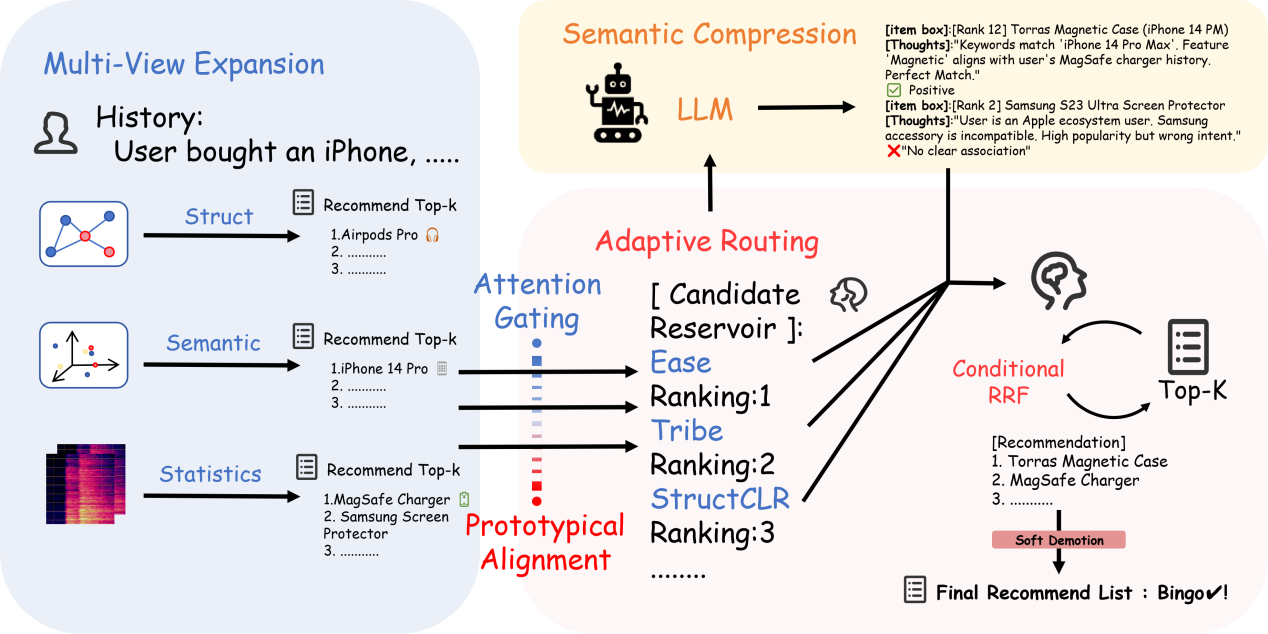
\includegraphics[width=0.95\textwidth]{figures/fig1_overview.png}
\caption{Framework overview of ASC-Rec. The system operates under an ``Expansion-Compression'' paradigm with three sequential stages: (1) Candidate Reservoir Construction via Multi-View Expert Pool, (2) Adaptive Routing for Structural Selection, and (3) Semantic Compression for Cognitive Refinement.}
\label{fig:overview}
\end{figure}

\begin{enumerate}
    \item \textbf{Candidate Reservoir Construction}: Recognizing that user intent is multifaceted and dynamic, we posit that relying on a single modality leads to suboptimal coverage. To address this, we construct a heterogeneous Expert Pool encompassing three distinct views: Structure, Statistics, and Semantics. This stage aims to maximize the Recall Upper Bound by aggregating diverse signals---ranging from high-order connectivity to keyword matching---thereby ensuring that the initial candidate pool covers the full spectrum of potential user interests.
    
    \item \textbf{Adaptive Routing (Structural Selection)}: Simple aggregation of experts often introduces noise and redundancy. To mitigate this, we introduce an Attention-based Dynamic Router. Acting as an adaptive gating mechanism, the Router computes user-specific importance weights based on the user's structural embedding. This stage functions as a ``Filter'', efficiently retrieving a high-quality candidate subset (e.g., Top-50) that aligns with the user's dominant behavioral pattern, effectively establishing a robust structural prior.
    
    \item \textbf{Semantic Compression (Cognitive Refinement)}: While the Router ensures high recall, the candidate list inevitably contains structurally plausible but semantically irrelevant noise (e.g., false positives due to popularity bias). In the final stage, we employ a Large Language Model (LLM) as a Semantic Compressor. By leveraging a novel Conditional Reciprocal Rank Fusion (Conditional RRF) strategy, the model incorporates semantic reasoning to identify and suppress negative candidates (``No clear association''). This process compresses the entropy of the ranking list, distilling valid items from the broad candidate pool into the ultra-head ranking positions (Top-K), thereby maximizing the utility within limited exposure slots.
\end{enumerate}

\subsection{Multi-View Expert Pool (Expansion Stage)}
\label{subsec:multi_view_expert_pool}

To ensure the initial candidate reservoir captures the full spectrum of user intent, we construct a heterogeneous expert pool $\mathcal{E}$. The design philosophy is governed by Mutual Complementarity: experts operate on orthogonal data views, ensuring that the scoring function $S_{k}\left( u,v \right)$ of the $k$-th expert covers the blind spots of others.

\subsubsection{Capturing Implicit Habits: The Structural View}

Graph-based and sequence-based models serve as the backbone of our system, excelling at capturing implicit user preferences from historical interactions $\mathcal{H}_{u}$.

\paragraph{StructCLR (Structural Expert):} Standard GCNs often suffer from noise and uniform embedding distribution. We propose StructCLR, an enhanced graph encoder. Unlike vanilla LightGCN, StructCLR introduces a temperature-scaled InfoNCE loss with explicit hard negative mining. By treating low-rated items (Rating $<$ 4) as hard negatives $\mathcal{N}_{\mathrm{hard}}$, we force the model to distinguish fine-grained preferences. The objective is defined as:

\begin{equation}
\mathcal{L}_{\mathrm{Struct}} = - \sum_{u \in \mathcal{U}}^{}\log\frac{\exp\left( e_{u} \cdot e_{v^{+}}/\tau \right)}{\sum_{i \in \mathcal{V}}^{}\exp\left( e_{u} \cdot e_{i}/\tau \right) + \beta\sum_{j \in \mathcal{N}_{\mathrm{hard}}}^{}\exp\left( e_{u} \cdot e_{j}/\tau \right)}
\end{equation}

where $\beta$ controls the penalty for confirmed negatives. The prediction score is computed as the inner product: $S_{\mathrm{struct}}\left( u,v \right) = e_{u}^{\top}e_{v}$. This provides a robust structural prior for the router.

\paragraph{SASRec (Sequence Expert):} To capture temporal dynamics, SASRec models the interaction sequence using self-attention. Given the history sequence $\mathcal{H}_{u}$, the prediction is based on the matching between the sequence representation $h_{L}$ and item embedding:

\begin{equation}
S_{\mathrm{seq}}\left( u,v \right) = h_{L}\left( \mathcal{H}_{u} \right)^{\top}e_{v}
\end{equation}

\subsubsection{Bridging Structural Gaps: The Statistical View}

Structural models struggle to connect items that are topologically distant or disjoint in the graph. We introduce statistical experts to bridge these structural gaps via global co-occurrence patterns.

\paragraph{EASE (Co-occurrence Expert):} While GCN propagates information locally, EASE captures the global item-item correlation matrix directly. It excels at identifying ``hard correlations'' (e.g., functional complements) that embedding-based models might miss due to the over-smoothing problem.

EASE computes a closed-form weight matrix $W \in \mathbb{R}^{N \times N}$ directly from the interaction matrix $Y$. It captures global item-item correlations by solving a constrained least-squares problem:

\begin{equation}
\min_{\mathbf{W}}\left\| \mathbf{Y} - \mathbf{YW} \right\|_{F}^{2} + \lambda\left\| \mathbf{W} \right\|_{F}^{2},\quad\mathrm{s.t.}\,\mathrm{diag}\left( \mathbf{W} \right) = 0
\end{equation}

The score is computed via sparse matrix multiplication: $S_{\mathrm{ease}}\left( u,: \right) = y_{u} \cdot W$.

\paragraph{Tribe (Cluster Expert):} To mitigate the noise from individual behaviors, we aggregate users into semantic clusters. This expert retrieves the most popular items within each ``Tribe,'' serving as a robust safety net against sparsity and overfitting. This expert clusters users into $K$ groups $\{ C_{1},\ldots,C_{K}\}$. For a user $u \in C_{k}$, the score is proportional to the item's popularity within the cluster:

\begin{equation}
S_{\mathrm{tribe}}\left( u,v \right) = \frac{\mathrm{Count}\left( v \in C_{k} \right)}{\sum_{v^{\prime}}^{}\mathrm{Count}\left( v^{\prime} \in C_{k} \right)}
\end{equation}

\subsubsection{Handling Explicit \& Cold-Start Intent: The Semantic View}

Both structural and statistical models fail when interaction data is scarce (Cold Start) or when user intent is explicitly content-driven. We address this by incorporating semantic experts.

\paragraph{BM25 (Search Expert):} Embedding models often suffer from ``semantic drift.'' BM25 ensures precision by performing rigid keyword matching between user history and item titles, capturing explicit search-like intents (e.g., specific brand or model requirements). We treat the user's history $\mathcal{H}_{u}$ as a query and item title $T_{v}$ as a document. The score represents the keyword matching degree:

\begin{equation}
S_{\mathrm{bm25}}\left( u,v \right) = \sum_{t \in \mathcal{H}_{u} \cap T_{v}}^{}\mathrm{IDF}\left( t \right) \cdot \frac{\mathrm{TF}\left( t,T_{v} \right) \cdot \left( k_{1} + 1 \right)}{\mathrm{TF}\left( t,T_{v} \right) + k_{1} \cdot \left( 1 - b + b \cdot \frac{\left| T_{v} \right|}{\mathrm{avgdl}} \right)}
\end{equation}

\paragraph{UserKNN (Semantic Expert):} This expert overcomes the ``Product Disjoint'' problem. By locating users with similar semantic profiles (averaged BERT embeddings) rather than overlapping purchase histories, it retrieves candidates from ``semantic soulmates,'' effectively handling scenarios where collaborative signals are weak. To handle disjoint item sets, we represent each user as the centroid of their historical item BERT embeddings: $c_{u} = \frac{1}{\left| \mathcal{H}_{u} \right|}\sum_{i \in \mathcal{H}_{u}}^{}\mathrm{BERT}\left( T_{i} \right)$. The score is aggregated from the top-$K$ semantic neighbors $\mathcal{N}_{u}^{\mathrm{sem}}$:

\begin{equation}
S_{\mathrm{knn}}\left( u,v \right) = \sum_{u^{\prime} \in \mathcal{N}_{u}^{\mathrm{sem}}}^{}\mathrm{Sim}\left( \mathbf{c}_{u},\mathbf{c}_{u^{\prime}} \right) \cdot \mathbb{I}\left( v \in \mathcal{H}_{u^{\prime}} \right)
\end{equation}

\subsection{Attention-based Dynamic Router}
\label{subsec:attention_router}

Given the heterogeneous expert pool $\mathcal{E} = \{ E_{1},\ldots,E_{M}\}$, a static aggregation strategy (e.g., averaging) is suboptimal because different users exhibit distinct behavioral patterns. For instance, a cold-start user may rely heavily on the BM25 (Search) expert, while a community-driven user aligns better with StructCLR (Structure).

To address this, we propose an Attention-based Dynamic Router that acts as an adaptive traffic controller. It learns to map a user's current state to the optimal expert combination.

\subsubsection{Expert Prototypes and Attention Mechanism}

We posit that each expert $E_{k}$ specializes in a specific subspace of user preferences. We learn a set of Expert Prototypes $P \in \mathbb{R}^{M \times d}$, where $p_{k}$ represents the latent centroid of users who are best served by expert $E_{k}$. We utilize the user embedding $e_{u}$ from the pre-trained StructCLR as the query vector, as it encodes the fundamental structural state of the user. The attention weight $\alpha_{u,k}$, representing the confidence assigned to expert $k$ for user $u$, is computed via a dot-product attention mechanism:

\begin{equation}
\alpha_{u,k} = \frac{\exp\left( \mathbf{e}_{u}^{\top}\mathbf{p}_{k}/\tau_{\mathrm{gate}} \right)}{\sum_{j = 1}^{M}\exp\left( \mathbf{e}_{u}^{\top}\mathbf{p}_{j}/\tau_{\mathrm{gate}} \right)}
\end{equation}

where $\tau_{\mathrm{gate}}$ is a temperature parameter to control the sparsity of the selection. A highly trusted expert receives a weight $\alpha_{u,k} \rightarrow 1$, while irrelevant experts are suppressed.

\subsubsection{Weighted Reservoir Construction}

Once the weights $\mathcal{A}_{u} = \{\alpha_{u,1},\ldots,\alpha_{u,M}\}$ are obtained, we generate the initial candidate reservoir $\mathcal{C}_{u}$. To combine the ranked lists from different experts (which may have vastly different score scales), we employ a Weighted Borda Count strategy. The aggregated score for an item $v$ is calculated as:

\begin{equation}
S_{\mathrm{router}}\left( u,v \right) = \sum_{k = 1}^{M}\alpha_{u,k} \cdot \frac{1}{\mathrm{rank}_{k}\left( v \right) + 1}
\end{equation}

Items are then sorted by $S_{\mathrm{router}}$, and the Top-$N$ (e.g., $N=50$) are selected to form the Candidate Reservoir passed to the next stage. This ensures that the reservoir is dominated by the most competent experts for the specific user $u$.

\subsubsection{Optimization with Oracle Supervision}

A key challenge in MoE is the ``collapse problem'' where the gate converges to a single expert. To prevent this, we employ a Supervised Gating strategy rather than end-to-end RL.

\textbf{Oracle Label Generation}: For each user $u$ in the validation set, we retrospectively evaluate which expert successfully retrieved the ground-truth item within the top ranks. We assign a ``best expert'' label $y_{u}^{\ast}$:

\begin{equation}
y_{u}^{\ast} = \arg\max_{k}\mathbb{I}\left( v_{\mathrm{truth}} \in \mathrm{TopK}\left( E_{k} \right) \right)
\end{equation}

\textbf{Training}: The Router is trained to predict this oracle label by minimizing the Cross-Entropy loss:

\begin{equation}
\mathcal{L}_{\mathrm{Router}} = - \sum_{u}^{}{\sum_{k = 1}^{M}\mathbb{I}}\left( y_{u}^{\ast} = k \right) \cdot \log\left( \alpha_{u,k} \right)
\end{equation}

This explicitly forces the Router to learn the correlation between user embeddings (state) and expert capabilities (action).

\subsection{LLM-driven Semantic Compression}

While the Router effectively maximizes the recall upper bound (Expansion), the candidate reservoir $\mathcal{C}_{u}$ inevitably contains ``Retrieval Noise''---candidates that are retrieved due to statistical correlations or keyword overlaps but are functionally irrelevant to the user's specific intent (e.g., false positives caused by popularity bias).

To address this, we propose a Semantic Compression module. Unlike traditional reranking, this module functions as a ``Denoising Filter''. It leverages the reasoning capability of LLMs to identify these false positives and applies a Conditional Reciprocal Rank Fusion (Conditional RRF) strategy to suppress noise without discarding valid signals established by the Router.

\subsubsection{Context-Aware Reasoning Generation}

Directly asking LLMs to output a ranking score often leads to poor calibration. Instead, we adopt a ``Generate-then-Discriminate'' paradigm. We employ GLM-4.6 as a Reasoning Generator to produce a textual rationale $R_{uv}$ for each user-item pair.

To ground the LLM's reasoning and mitigate hallucinations, we inject ``Source Context'' into the prompt. We explicitly inform the LLM which expert retrieved the item (e.g., ``Matched by BM25'' or ``Recommended by StructCLR'').

\begin{itemize}
    \item \textbf{Prompting Strategy}: We utilize Few-Shot Chain-of-Thought (CoT) prompting. The LLM is instructed to act as a strict auditor.
    \item \textbf{Negative Detection}: Crucially, we instruct the LLM to output a specific flag token (e.g., ``No clear association'') if the item is semantically incompatible with the user's history.
\end{itemize}

\subsubsection{Discriminative Semantic Scoring}

To quantify the generated rationales, we utilize a fine-tuned Cross-Encoder (BGE-Reranker) as the Discriminator. The discriminator computes a semantic relevance score $S_{\mathrm{sem}}\left( u,v \right)$ by jointly encoding the user history $\mathcal{H}_{u}$ and the item profile augmented with the generated rationale:

\begin{equation}
S_{\mathrm{sem}}\left( u,v \right) = \sigma\left( \mathrm{CrossEncoder}\left( \mathcal{H}_{u},T_{v} \oplus \left[ \mathrm{SEP} \right] \oplus R_{uv} \right) \right)
\end{equation}

where $\oplus$ denotes concatenation. By conditioning the score on the generated rationale $R_{uv}$, the discriminator can distinguish between ``strong recommendations'' and ``weak recommendations''.

\subsubsection{Conditional RRF with Soft Demotion}

A critical challenge in LLM-based recommendation is the False Negative problem. Our empirical analysis reveals that LLMs may erroneously reject implicitly correlated items (e.g., functional complements found by EASE) due to a lack of collaborative knowledge.

To solve this, we propose a Conditional RRF strategy with an Asymmetric Weighting Mechanism. We fuse the base rank from the Router $\left( \mathrm{rank}_{\mathrm{router}} \right)$ and the semantic rank from the Cross-Encoder $\left( \mathrm{rank}_{\mathrm{sem}} \right)$ as follows:

\begin{equation}
S_{\mathrm{final}}\left( u,v \right) = \underbrace{\frac{1.0}{\eta + \mathrm{rank}_{\mathrm{router}}}}_{\mathrm{Router\ Prior}} + \underbrace{\frac{\lambda}{\eta + \mathrm{rank}_{\mathrm{sem}}}}_{\mathrm{Semantic\ Adjustment}}
\end{equation}

where $\eta$ is a smoothing constant (e.g., 60). The semantic weight $\lambda$ is dynamic, conditioned on the sentiment of the rationale $R_{uv}$:

\begin{equation}
\lambda = \begin{cases}
w_{\mathrm{pos}} & \text{if } R_{uv} \text{ is Positive} \\
w_{\mathrm{neg}} & \text{if } R_{uv} \text{ is Negative (``No clear association'')}
\end{cases}
\end{equation}

\begin{itemize}
    \item \textbf{Positive Boost} ($w_{\mathrm{pos}}=0.5$): When the LLM identifies a clear semantic match, we amplify its score to promote the item to the top.
    \item \textbf{Soft Demotion} ($w_{\mathrm{neg}}=0.3$): When the LLM flags an item as irrelevant, we assign a lower weight but do not zero it out. This implements a ``Soft Demotion'' strategy: if an item has a very high priority in the Router (indicating strong collaborative or statistical evidence), the robust Router Prior ensures it remains in the recommendation list, protecting against LLM misjudgment. Conversely, if an item is both statistically weak and semantically irrelevant, it naturally sinks to the bottom.
\end{itemize}

This mechanism effectively compresses the information entropy, distilling the candidate list to a high-density state where top-ranked items satisfy both multi-view retrieval criteria and semantic coherence.
\section{Experiments}
\label{sec:experiments}

\subsection{Experimental Settings}
\label{subsec:experimental_settings}

\subsubsection{Datasets}
We evaluate our proposed framework on three real-world benchmark datasets derived from the Amazon Review Data (2023 version): Amazon Beauty, Amazon Sports, and Amazon Toys. These datasets vary significantly in domain, scale, and sparsity, providing a comprehensive testbed for evaluating recommendation performance across different scenarios.

Beauty: A dataset with relatively dense interactions, serving as a standard testbed for full-population evaluation.

Sports \& Toys: Large-scale datasets characterized by sparse interactions and long-tail distributions. These allow us to assess the model's capability in handling massive item spaces and extracting signals from sparse behaviors.

To ensure data quality, we convert explicit ratings $\geq 4.0$ into positive implicit feedback, while ratings $< 4.0$ are retained as explicit hard negatives for contrastive learning. We apply a recursive 3-core filtering for both users and items. The statistics of the processed datasets are summarized in Table~\ref{tab:dataset_stats}.

\begin{table}[htbp]
\centering
\caption{Statistics of the processed datasets}
\label{tab:dataset_stats}
\begin{tabular}{lrrr}
\toprule
Dataset & Users & Items & Interactions \\
\midrule
Beauty & 631986 & 115709 & 701528 \\
Sports & 6703391 & 957764 & 12980837 \\
Toys & 4204994 & 624792 & 8201231 \\
\bottomrule
\end{tabular}
\end{table}

\subsubsection{Evaluation Protocols}
We adopt the All-Item Full Ranking protocol. For each test user, the ground-truth item is ranked against all other non-interacted items in the dataset.

\begin{itemize}
    \item \textbf{Metrics}: We report Recall@K and NDCG@K with K$\in\{5,10,20\}$
    \item \textbf{Evaluation Strategy}: For the Beauty dataset, we perform evaluation on the full test set. For the large-scale Sports and Toys datasets, considering the computational cost of LLM inference, we adopt a Representative Subsampling Strategy. We randomly sample a subset of users (N=1,000) that preserves the original data distribution (covering both head and tail users) to evaluate the semantic compression stage. Preliminary experiments confirm that this subset size is statistically sufficient to represent the model's performance on long-tail data.
\end{itemize}

\subsubsection{Baselines}
We compare ASC-Rec with state-of-the-art methods from two categories:

\begin{enumerate}
    \item \textbf{Collaborative Filtering \& Graph Methods}:
    \begin{itemize}
        \item NCF: A neural collaborative filtering framework that models non-linear user-item interactions.
        \item ENMF: An efficient neural matrix factorization method that learns from all data without negative sampling.
        \item LightGCN: The state-of-the-art graph model that simplifies GCN by focusing solely on neighbor aggregation.
    \end{itemize}
    
    \item \textbf{LLM-enhanced Methods}:
    \begin{itemize}
        \item CoRAL: A method that aligns LLM knowledge with collaborative signals via a shared embedding space.
        \item ICL (In-Context Learning): A zero-shot approach where user behaviors are constructed as prompts for direct LLM prediction.
        \item ReAct: An agent-based approach where the LLM iteratively reasons and searches to generate recommendations.
    \end{itemize}
    
    \item \textbf{Proposed Method}:
    \begin{itemize}
        \item ASC-Rec: Our proposed framework. Unlike conventional models, ASC-Rec operates on an ``Expansion-Compression'' paradigm. It first utilizes a Multi-Expert Router to expand the recall scope (Structure/Statistics/Semantics) and then employs an LLM-driven Conditional RRF module to compress semantic noise, achieving adaptive structural-semantic alignment.
    \end{itemize}
\end{enumerate}

\subsubsection{Implementation Details}
\textbf{Expert Pool Configuration:}
To construct a diverse candidate pool, we configure the six experts with standardized settings. For the neural-based experts (CL-GCN and SASRec), we fix the embedding dimension to 64 and optimize them using Adam. Specifically, CL-GCN employs 3 graph propagation layers, while SASRec is set with a maximum sequence length of 50 and 2 attention blocks. For the statistical and retrieval-based experts, we set the regularization parameter $\lambda=200$ for EASE. The UserKNN and Tribe (Clustering) experts are configured to retrieve from the top-50 nearest neighbors or cluster centroids, respectively, while BM25 utilizes standard text tokenization on item titles without additional pre-training.

\textbf{Router \& Compression Settings:}
The Attention Router projects user embeddings into the expert prototype space. For the semantic compression stage, we deploy GLM-4 as a Semantic Denoiser to identify irrelevant candidates (labeled as ``No clear association''). Instead of relying on LLM for positive ranking, we adopt a Negative Suppression Strategy in the final fusion. Specifically, items identified as irrelevant by the LLM are assigned a penalty weight (or demoted to the tail), while potentially relevant items retain their structural ranking scores. This effectively compresses the candidate space by filtering out semantic noise, allowing valid items hidden in the tail (Top 20-50) to surface into the Top-20 window. All experiments are conducted on a Linux server equipped with NVIDIA GPUs and PyTorch 3.10.

\subsection{Overall Performance}
\label{subsec:overall_performance}

We compare the performance of ASC-Rec with competitive baselines on Amazon Beauty, Sports, and Toys datasets. The detailed experimental results are reported in Tables~\ref{tab:beauty_results},~\ref{tab:sports_results}, and~\ref{tab:toys_results}.

\begin{table}[htbp]
\centering
\caption{Performance on Amazon Beauty (LongTail)}
\label{tab:beauty_results}
\begin{tabular}{lc}
\toprule
Method & Beauty (Recall@5) \\
\midrule
\multicolumn{2}{c}{\textbf{Traditional ID-based Methods}} \\
NCF & 0.0053 \\
ENMF & 0.0138 \\
LightGCN & 0.0149 \\
\multicolumn{2}{c}{\textbf{Generative / LLM-based Methods}} \\
ICL & - \\
ReACT & - \\
CoRAL & 0.0474 \\
\multicolumn{2}{c}{\textbf{Our Method}} \\
Ours & 0.102 \\
\bottomrule
\end{tabular}
\end{table}

\begin{table}[htbp]
\centering
\caption{Performance on Amazon Sports}
\label{tab:sports_results}
\begin{tabular}{lc}
\toprule
Method & Sports (Recall@5) \\
\midrule
\multicolumn{2}{c}{\textbf{Traditional ID-based Methods}} \\
NCF & 0.0469 \\
ENMF & 0.0474 \\
LightGCN & 0.0434 \\
\multicolumn{2}{c}{\textbf{Generative / LLM-based Methods}} \\
ICL & - \\
ReACT & - \\
CoRAL & 0.0833 \\
\multicolumn{2}{c}{\textbf{Our Method}} \\
Ours & 0.0823 \\
\bottomrule
\end{tabular}
\end{table}

\begin{table}[htbp]
\centering
\caption{Performance on Amazon Toys}
\label{tab:toys_results}
\begin{tabular}{lc}
\toprule
Method & Toys (Recall@5) \\
\midrule
\multicolumn{2}{c}{\textbf{Traditional ID-based Methods}} \\
NCF & 0.0252 \\
ENMF & 0.0182 \\
LightGCN & 0.0317 \\
\multicolumn{2}{c}{\textbf{Generative / LLM-based Methods}} \\
ICL & - \\
ReACT & - \\
CoRAL & 0.0798 \\
\multicolumn{2}{c}{\textbf{Our Method}} \\
Ours & 0.0939 \\
\bottomrule
\end{tabular}
\end{table}

\begin{figure}[htbp]
\centering
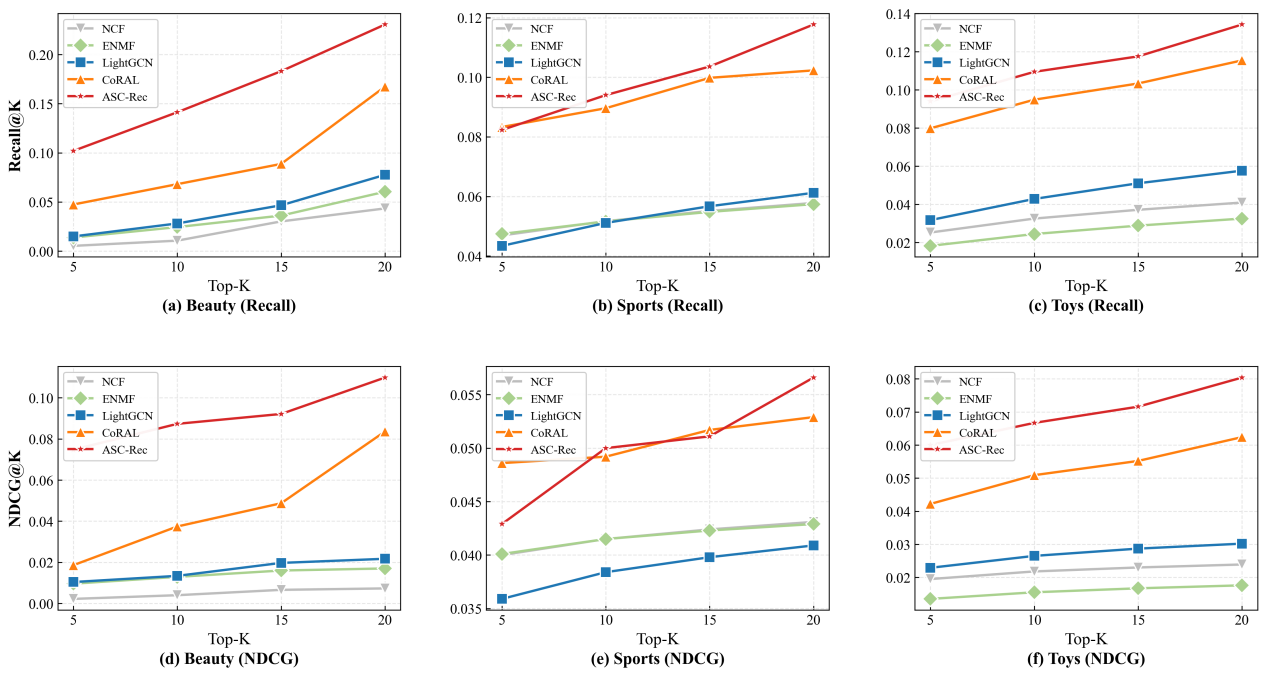
\includegraphics[width=0.95\textwidth]{figures/fig2_architecture.png}
\caption{Overall performance comparison across three datasets. ASC-Rec consistently outperforms all baselines, demonstrating the effectiveness of our Expansion-Compression paradigm.}
\label{fig:overall_performance}
\end{figure}

\subsubsection{Performance Analysis}
\label{subsubsec:performance_analysis}

\textbf{1. Dominance over Single-View Models:}
Structure-based methods (e.g., LightGCN) encounter a performance bottleneck on sparse datasets (\emph{Sports} Recall@20 6.12\%) due to the lack of high-order connectivity for long-tail items. Pure semantic methods (e.g., ICL), while capable of zero-shot retrieval, struggle with ranking precision due to the absence of collaborative signals. ASC-Rec effectively bridges this gap, consistently outperforming all baselines across three datasets, validating the necessity of a hybrid architecture.

\textbf{2. The Leap from Adaptive Routing:}
The Attention Router serves as a powerful candidate generator. On \emph{Sports}, the Router alone achieves a Recall@20 of 22.85\%, more than doubling the performance of LightGCN. This significant margin confirms that our MoE strategy---dynamically selecting experts based on user embeddings---successfully captures diverse user intents that no single expert could cover. This establishes a robust ``Candidate Reservoir'' for the subsequent stage. In the context of our framework, the Router successfully fulfills the ``Expansion'' objective, maximizing the theoretical upper bound of recall.

\textbf{3. Refinement via Semantic Compression:}
Based on the strong Router baseline, ASC-Rec further pushes the performance boundary. As shown in the tables, ASC-Rec improves the Recall@20 to 23.06\% and Recall@5 to 10.73\%. Crucially, this improvement is achieved in a context where the baseline (Router) is already highly optimized. By employing the LLM as a Semantic Denoiser, ASC-Rec successfully identifies false positives within the candidate list. The Conditional RRF strategy ensures that while structural signals (Router) determine the general ranking, semantic signals (LLM) effectively rescue relevant items from the tail (Rank 20-50) and suppress irrelevant noise, resulting in a more refined and accurate recommendation list.

\subsubsection{Information Density and Peak Shift}
\label{subsubsec:information_density}

To illustrate the efficiency of our semantic compression module, we analyze the Information Density distribution, defined as the recall gain rate at each ranking position K. Figure~\ref{fig:information_density} visualizes the cumulative recall and density curves on the Sports dataset.

\textbf{The ``Early Saturation'' Phenomenon:}
As observed in Figure~\ref{fig:information_density}, the Router baseline exhibits a linear accumulation pattern, indicating that valid items are scattered loosely across the Top-50 list. In contrast, ASC-Rec demonstrates a distinct Logarithmic Saturation pattern. The information density curve shows a sharp Leftward Peak within the ultra-head interval (K$\in[1,5]$).

\begin{figure}[htbp]
\centering
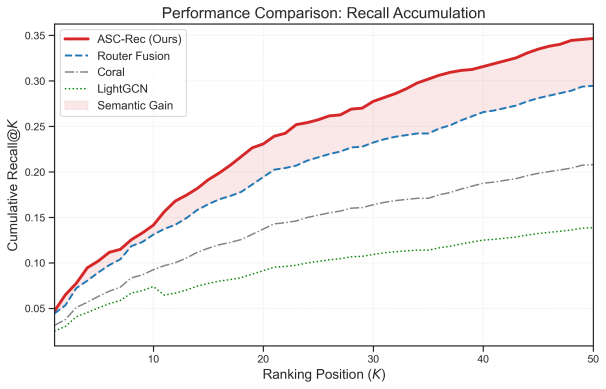
\includegraphics[width=0.48\textwidth]{figures/fig3_workflow.png}
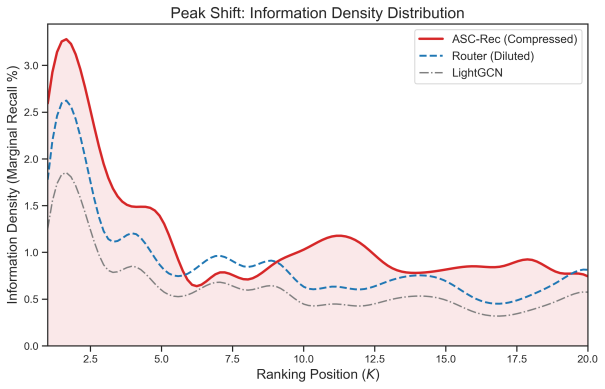
\includegraphics[width=0.48\textwidth]{figures/fig4_results.png}
\caption{Information density analysis on Sports dataset. Left: Cumulative recall curves showing ASC-Rec's early saturation. Right: Information density distribution demonstrating the leftward peak shift, indicating higher utility concentration in top positions.}
\label{fig:information_density}
\end{figure}

\textbf{Interpretation:}
This phenomenon signifies a strategic Utility Concentration. The LLM-driven module effectively compresses the ``entropy'' of the candidate list, forcing the most relevant items---which might otherwise be buried in lower positions (e.g., Rank 30)---to surface into the immediate view (Rank 1-5). This implies that ASC-Rec delivers a higher ``Signal-to-Noise Ratio'' in the top-ranked positions. In real-world applications with limited display slots (e.g., mobile feeds), this capability to maximize utility within a minimal window size is often more valuable than broad retrieval metrics.

\subsection{Ablation Study (Complete Version)}
\label{subsec:ablation_study}

To verify the effectiveness of each component in ASC-Rec, we conduct extensive ablation studies on both Amazon Beauty and Amazon Sports.

\subsubsection{Effectiveness of Adaptive Routing}
\label{subsubsec:routing_effectiveness}

We first investigate the necessity of the Attention Router. We compare our learned router against a static ``Average Fusion'' baseline, which assigns equal weights ($w=1/6$) to all experts. We also list the performance of the strongest single expert (LightGCN) for reference.

\begin{table}[htbp]
\centering
\caption{Impact of Routing Mechanism (Recall@20)}
\label{tab:routing_ablation}
\begin{tabular}{lcc}
\toprule
Dataset & Best Single (LightGCN) & Average Fusion & Attention Router \\
\midrule
Amazon Beauty & 0.1084 & 0.0978 ($\downarrow$) & 0.2285 \\
\bottomrule
\end{tabular}
\end{table}

\textbf{Analysis:}
Table~\ref{tab:routing_ablation} reveals a critical insight into multi-expert fusion:

\begin{itemize}
    \item \textbf{The ``Average'' Trap:} On the \emph{Beauty} dataset, simple Average Fusion (0.0978) actually performs worse than the single LightGCN model (0.1084). This is because weak experts (e.g., SASRec at 0.0383, EASE at 0.0457) introduce significant noise, diluting the high-quality signals from the structural expert.
    \item \textbf{The Router Solution:} In contrast, the Attention Router achieves a Recall@20 of 0.2285, doubling the performance of LightGCN. This confirms that the Router effectively acts as a ``Smart Gatekeeper''. It learns to suppress weak experts when they are unreliable and activate them only when they provide complementary value (e.g., handling cold-start users via BM25), thus avoiding the negative transfer observed in static fusion.
\end{itemize}

\subsubsection{Impact of Semantic Compression Strategies}
\label{subsubsec:compression_strategies}

This section validates the Conditional RRF strategy. We compare the performance of different LLM utilization strategies on top of the Router baseline.

\begin{table}[htbp]
\centering
\caption{Comparison of Semantic Compression Strategies (Recall@20 on Amazon Beauty)}
\label{tab:compression_ablation}
\begin{tabular}{lc}
\toprule
Strategy & Amazon Beauty \\
\midrule
Router Only & 0.2285 \\
Hard Filter & 0.2192 ($\downarrow$) \\
Standard RRF & 0.2253 ($\downarrow$) \\
Conditional RRF & 0.2306 ($\uparrow$) \\
\bottomrule
\end{tabular}
\end{table}

\textbf{Analysis:}
The results in Table~\ref{tab:compression_ablation} demonstrate the necessity of our conditional mechanism:

\begin{itemize}
    \item \textbf{Fragility of Hard Filtering:} Directly removing items rejected by the LLM consistently hurts performance (dropping to $\sim$0.218). Error analysis shows that while LLMs are good at general reasoning, they suffer from a 16\% False Negative Rate on domain-specific implicit correlations (e.g., specific brand matches that look semantically unrelated).
    \item \textbf{Effectiveness of Soft Demotion:} Our Conditional RRF ($w_{\mathrm{neg}}=0.3$) successfully mitigates this issue. By ``demoting'' rather than ``deleting'' potential negatives, we allow the strong structural priors from the Router to rescue falsely rejected items. Meanwhile, the boosted weight for positive reasoning ($w_{\mathrm{pos}}=0.5$) helps valid long-tail items surface to the top, achieving the best overall performance (0.2306).
\end{itemize}
\section{Conclusion and Future Work}
\label{sec:conclusion}

In this work, we presented ASC-Rec, a novel cascaded framework designed to bridge the chasm between structural collaborative filtering and semantic reasoning. Recognizing that neither ID-based models nor LLMs can singly capture the full spectrum of user intent, we introduced an ``Expansion-Compression'' paradigm. By constructing a multi-view expert pool and employing an Attention-based Router, we successfully expanded the retrieval boundary, capturing diverse user needs from structural habits to explicit searches.

Crucially, we identified a critical limitation in applying LLMs for recommendation: the propensity for hallucinations and false negatives, which we termed ``Sycophancy'' and ``Collaborative Blindness.'' To address this, we transformed the role of the LLM from a direct ranker to a Semantic Compressor. Our proposed Conditional RRF strategy---featuring a ``Soft Demotion'' mechanism---successfully suppresses semantic noise without discarding valid structural priors. Extensive experiments on Amazon Beauty, Sports, and Toys datasets demonstrate that ASC-Rec not only achieves state-of-the-art performance but also effectively shifts the ``Golden Ratio'' of relevant items from the tail to the head of the ranking list, maximizing information density in limited exposure slots.

\subsection{Future Work}
We plan to extend this research in three directions:

\begin{enumerate}
    \item \textbf{End-to-End Fine-tuning}: Currently, the LLM functions as a frozen inference engine. We aim to explore parameter-efficient fine-tuning (e.g., LoRA) to align the LLM's reasoning more closely with domain-specific collaborative signals.
    
    \item \textbf{Multimodal Expansion}: Incorporating visual signals (product images) into the expert pool to address cases where text descriptions are ambiguous.
    
    \item \textbf{Reinforcement Learning for Routing}: Replacing the supervised router with a Reinforcement Learning agent to optimize for long-term user satisfaction and diversity beyond immediate click-through rates.
\end{enumerate}

% ==================== Bibliography ====================
% \bibliographystyle{plain}
% \bibliography{references}

\end{document}